\section{Experiments and results}
\label{sec:experiments}

\subsection{Setup}
SKELETON

\subsection{Ablation studies of the traditional pipeline}
\subsubsection{Imputation}
\begin{table}[H]
\centering
\scriptsize
\begin{adjustbox}{max width=\linewidth}
\begin{tabular}{llrrrrrrr}
\toprule
model & imputer & indicator & pr\_auc & sd & roc\_auc & f2 & recall & precision \\
\midrule
Logistic Regression & mean & False & 0.6984 & 0.0046 & 0.8642 & 0.7061 & 0.7799 & 0.5122 \\
Logistic Regression & median & False & 0.6985 & 0.0045 & 0.8642 & 0.7063 & 0.7801 & 0.5125 \\
Logistic Regression & group\_median & False & 0.6989 & 0.0044 & 0.8643 & 0.7075 & 0.7806 & 0.5149 \\
Logistic Regression & knn & False & 0.6986 & 0.0045 & 0.8642 & 0.7059 & 0.7799 & 0.5117 \\
Logistic Regression & iterative & False & 0.6985 & 0.0046 & 0.8642 & 0.7061 & 0.7799 & 0.5122 \\
Logistic Regression & median & True & 0.6999 & 0.0052 & 0.8652 & 0.7079 & 0.7813 & 0.5145 \\
Random Forest & mean & False & 0.8835 & 0.0016 & 0.9324 & 0.7675 & 0.7381 & 0.9127 \\
Random Forest & median & False & 0.8827 & 0.0016 & 0.9313 & 0.7685 & 0.7392 & 0.9136 \\
Random Forest & group\_median & False & 0.8838 & 0.0017 & 0.9325 & 0.7691 & 0.7397 & 0.9144 \\
Random Forest & knn & False & 0.8839 & 0.0016 & 0.9321 & 0.7682 & 0.7380 & 0.9186 \\
Random Forest & iterative & False & 0.8836 & 0.0011 & 0.9322 & 0.7675 & 0.7376 & 0.9162 \\
Random Forest & median & True & 0.8824 & 0.0027 & 0.9316 & 0.7690 & 0.7404 & 0.9097 \\
\bottomrule
\end{tabular}
\end{adjustbox}
\caption{Imputation strategies: 5-fold CV on the training set (F2, recall and precision at threshold 0.5).}
\label{tab:suite_imputation}
\end{table}

\begin{figure}[H]\centering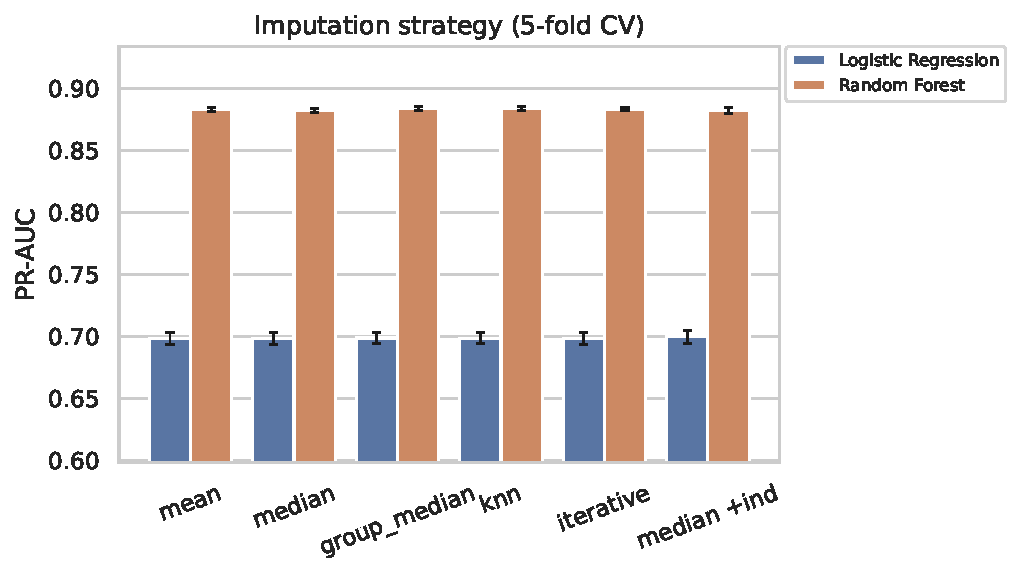
\includegraphics[width=0.9\linewidth]{suite_imputation.pdf}\caption{Imputation.}\label{fig:suite_imputation}\end{figure}
\subsubsection{Scaling}
\begin{table}[H]
\centering
\scriptsize
\begin{adjustbox}{max width=\linewidth}
\begin{tabular}{llrrrrrr}
\toprule
model & scaler & pr\_auc & sd & roc\_auc & f2 & recall & precision \\
\midrule
Logistic Regression & none & 0.6650 & 0.0098 & 0.8449 & 0.6884 & 0.7792 & 0.4696 \\
Logistic Regression & standard & 0.6985 & 0.0045 & 0.8642 & 0.7063 & 0.7801 & 0.5125 \\
Logistic Regression & minmax [0,1] & 0.6996 & 0.0048 & 0.8642 & 0.7066 & 0.7810 & 0.5120 \\
Logistic Regression & minmax [-1,1] & 0.6990 & 0.0049 & 0.8642 & 0.7069 & 0.7808 & 0.5129 \\
Logistic Regression & robust & 0.6986 & 0.0046 & 0.8642 & 0.7060 & 0.7798 & 0.5124 \\
k-NN & none & 0.6153 & 0.0109 & 0.8203 & 0.4926 & 0.4594 & 0.6949 \\
k-NN & standard & 0.7775 & 0.0072 & 0.8827 & 0.6114 & 0.5664 & 0.8964 \\
k-NN & minmax [0,1] & 0.7720 & 0.0072 & 0.8778 & 0.6098 & 0.5646 & 0.8972 \\
k-NN & minmax [-1,1] & 0.7723 & 0.0071 & 0.8779 & 0.6113 & 0.5662 & 0.8975 \\
k-NN & robust & 0.7708 & 0.0070 & 0.8820 & 0.5766 & 0.5288 & 0.9026 \\
SVM (RBF) & standard & 0.8340 & 0.0079 & 0.9075 & 0.7543 & 0.7674 & 0.7063 \\
SVM (RBF) & minmax [0,1] & 0.7966 & 0.0068 & 0.8967 & 0.7365 & 0.7644 & 0.6426 \\
SVM (RBF) & minmax [-1,1] & 0.8040 & 0.0071 & 0.9008 & 0.7433 & 0.7711 & 0.6496 \\
SVM (RBF) & robust & 0.8302 & 0.0082 & 0.9090 & 0.7581 & 0.7768 & 0.6918 \\
\bottomrule
\end{tabular}
\end{adjustbox}
\caption{Scaling methods: 5-fold CV on the training set (F2, recall and precision at threshold 0.5).}
\label{tab:suite_scaling}
\end{table}

\begin{figure}[H]\centering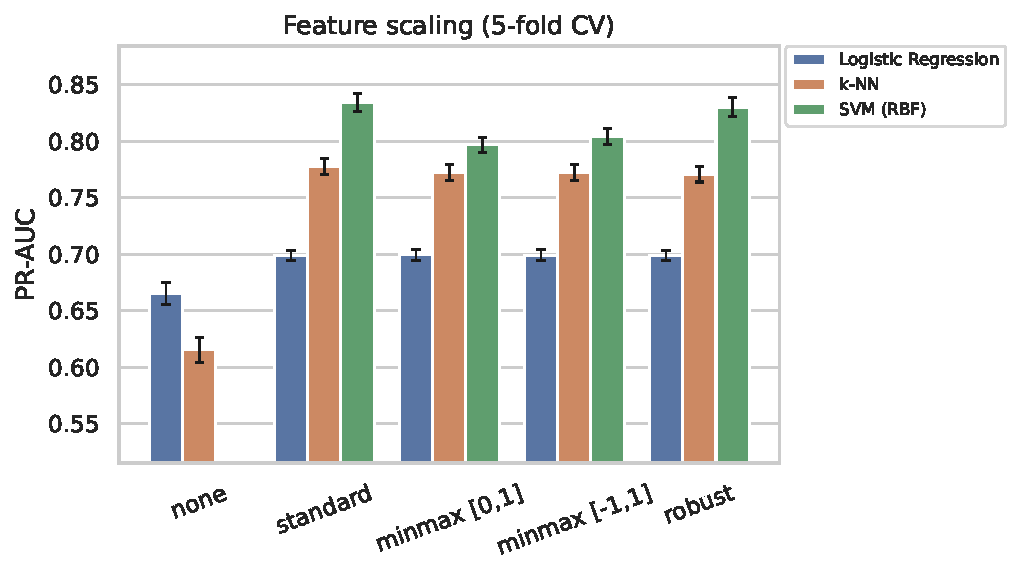
\includegraphics[width=0.9\linewidth]{suite_scaling.pdf}\caption{Scaling.}\label{fig:suite_scaling}\end{figure}
\subsubsection{Outliers and feature engineering}
\begin{table}[H]
\centering
\scriptsize
\begin{adjustbox}{max width=\linewidth}
\begin{tabular}{llrrrrrrr}
\toprule
model & outlier & feat\_eng & pr\_auc & sd & roc\_auc & f2 & recall & precision \\
\midrule
Logistic Regression & none & False & 0.6985 & 0.0045 & 0.8642 & 0.7063 & 0.7801 & 0.5125 \\
Logistic Regression & none & True & 0.7122 & 0.0037 & 0.8761 & 0.7221 & 0.7983 & 0.5226 \\
Logistic Regression & clip\_iqr & False & 0.7021 & 0.0049 & 0.8656 & 0.7082 & 0.7833 & 0.5120 \\
Logistic Regression & clip\_iqr & True & 0.7220 & 0.0053 & 0.8771 & 0.7273 & 0.8022 & 0.5297 \\
Logistic Regression & log & False & 0.7105 & 0.0040 & 0.8717 & 0.7133 & 0.7877 & 0.5179 \\
Logistic Regression & log & True & 0.7160 & 0.0035 & 0.8765 & 0.7227 & 0.7958 & 0.5285 \\
Random Forest & none & False & 0.8827 & 0.0016 & 0.9313 & 0.7685 & 0.7392 & 0.9136 \\
Random Forest & none & True & 0.8852 & 0.0011 & 0.9332 & 0.7721 & 0.7466 & 0.8942 \\
Random Forest & clip\_iqr & False & 0.8834 & 0.0020 & 0.9319 & 0.7690 & 0.7396 & 0.9146 \\
Random Forest & clip\_iqr & True & 0.8854 & 0.0011 & 0.9333 & 0.7718 & 0.7461 & 0.8951 \\
Random Forest & log & False & 0.8825 & 0.0018 & 0.9312 & 0.7685 & 0.7390 & 0.9143 \\
Random Forest & log & True & 0.8852 & 0.0011 & 0.9331 & 0.7721 & 0.7466 & 0.8942 \\
\bottomrule
\end{tabular}
\end{adjustbox}
\caption{Outlier handling and feature engineering: 5-fold CV on the training set (F2, recall and precision at threshold 0.5).}
\label{tab:suite_outlier_fe}
\end{table}

\begin{figure}[H]\centering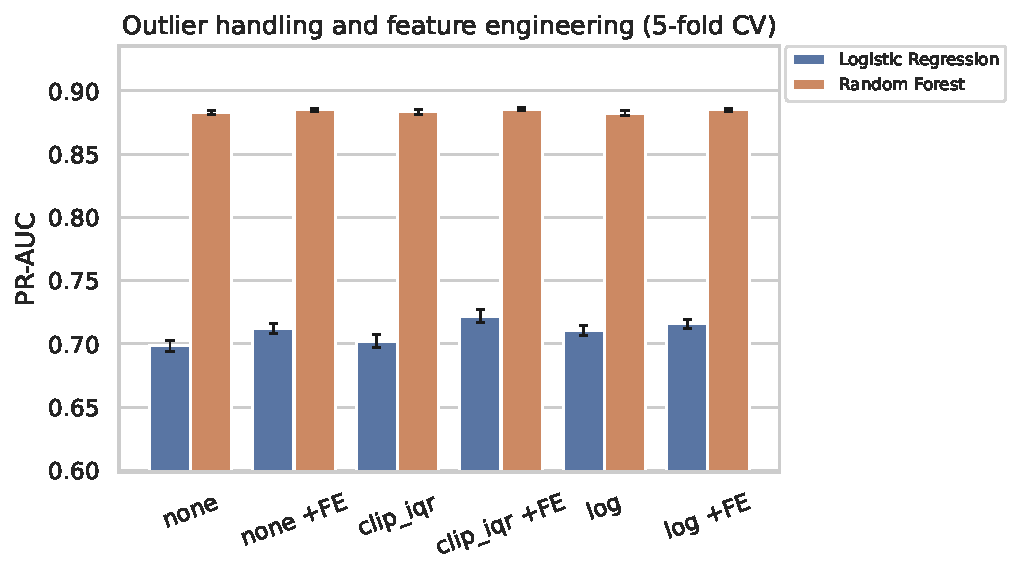
\includegraphics[width=0.9\linewidth]{suite_outlier_fe.pdf}\caption{Outliers.}\label{fig:suite_outlier_fe}\end{figure}
\subsubsection{Encoding}
\begin{table}[H]
\centering
\scriptsize
\begin{adjustbox}{max width=\linewidth}
\begin{tabular}{llrrrrrr}
\toprule
model & grade\_encoding & pr\_auc & sd & roc\_auc & f2 & recall & precision \\
\midrule
Logistic Regression & ordinal & 0.6985 & 0.0045 & 0.8642 & 0.7063 & 0.7801 & 0.5125 \\
Logistic Regression & onehot & 0.7165 & 0.0061 & 0.8708 & 0.7181 & 0.7791 & 0.5470 \\
k-NN & ordinal & 0.7775 & 0.0072 & 0.8827 & 0.6114 & 0.5664 & 0.8964 \\
k-NN & onehot & 0.7748 & 0.0083 & 0.8787 & 0.6179 & 0.5743 & 0.8871 \\
Random Forest & ordinal & 0.8827 & 0.0016 & 0.9313 & 0.7685 & 0.7392 & 0.9136 \\
Random Forest & onehot & 0.8819 & 0.0018 & 0.9309 & 0.7667 & 0.7392 & 0.9010 \\
\bottomrule
\end{tabular}
\end{adjustbox}
\caption{Encoding of the loan grade: 5-fold CV on the training set (F2, recall and precision at threshold 0.5).}
\label{tab:suite_encoding}
\end{table}

\subsubsection{Dimensionality}
\begin{table}[H]
\centering
\scriptsize
\begin{adjustbox}{max width=\linewidth}
\begin{tabular}{llrrrrrr}
\toprule
model & reduction & pr\_auc & sd & roc\_auc & f2 & recall & precision \\
\midrule
Logistic Regression & none & 0.6985 & 0.0045 & 0.8642 & 0.7063 & 0.7801 & 0.5125 \\
Logistic Regression & PCA 80\% & 0.6485 & 0.0095 & 0.8391 & 0.6867 & 0.7755 & 0.4711 \\
Logistic Regression & PCA 90\% & 0.6571 & 0.0048 & 0.8447 & 0.6869 & 0.7685 & 0.4824 \\
Logistic Regression & PCA 95\% & 0.6755 & 0.0086 & 0.8517 & 0.6957 & 0.7764 & 0.4915 \\
Logistic Regression & PCA 99\% & 0.6983 & 0.0046 & 0.8642 & 0.7064 & 0.7805 & 0.5123 \\
Logistic Regression & SelectKBest k=5 & 0.6693 & 0.0055 & 0.8475 & 0.6984 & 0.7798 & 0.4927 \\
Logistic Regression & SelectKBest k=10 & 0.6837 & 0.0053 & 0.8572 & 0.7007 & 0.7745 & 0.5075 \\
Logistic Regression & SelectKBest k=15 & 0.6920 & 0.0059 & 0.8614 & 0.7009 & 0.7739 & 0.5090 \\
k-NN & none & 0.7775 & 0.0072 & 0.8827 & 0.6114 & 0.5664 & 0.8964 \\
k-NN & PCA 80\% & 0.7251 & 0.0217 & 0.8648 & 0.5695 & 0.5317 & 0.7960 \\
k-NN & PCA 90\% & 0.7462 & 0.0092 & 0.8732 & 0.5939 & 0.5544 & 0.8304 \\
k-NN & PCA 95\% & 0.7550 & 0.0099 & 0.8755 & 0.5954 & 0.5528 & 0.8610 \\
k-NN & PCA 99\% & 0.7776 & 0.0070 & 0.8827 & 0.6112 & 0.5662 & 0.8958 \\
k-NN & SelectKBest k=5 & 0.7592 & 0.0045 & 0.8731 & 0.6281 & 0.5943 & 0.8136 \\
k-NN & SelectKBest k=10 & 0.7695 & 0.0077 & 0.8841 & 0.6429 & 0.6105 & 0.8170 \\
k-NN & SelectKBest k=15 & 0.7823 & 0.0110 & 0.8851 & 0.6258 & 0.5828 & 0.8890 \\
Random Forest & none & 0.8826 & 0.0017 & 0.9313 & 0.7677 & 0.7383 & 0.9133 \\
Random Forest & PCA 80\% & 0.7664 & 0.0296 & 0.8822 & 0.6810 & 0.6794 & 0.6880 \\
Random Forest & PCA 90\% & 0.8196 & 0.0074 & 0.9041 & 0.7096 & 0.6978 & 0.7612 \\
Random Forest & PCA 95\% & 0.8280 & 0.0073 & 0.9072 & 0.7148 & 0.7002 & 0.7800 \\
Random Forest & PCA 99\% & 0.8363 & 0.0076 & 0.9100 & 0.7300 & 0.7156 & 0.7945 \\
Random Forest & SelectKBest k=5 & 0.8301 & 0.0047 & 0.9053 & 0.7376 & 0.7374 & 0.7385 \\
Random Forest & SelectKBest k=10 & 0.8355 & 0.0068 & 0.9122 & 0.7463 & 0.7491 & 0.7359 \\
Random Forest & SelectKBest k=15 & 0.8684 & 0.0045 & 0.9253 & 0.7553 & 0.7369 & 0.8400 \\
\bottomrule
\end{tabular}
\end{adjustbox}
\caption{PCA and univariate feature selection: 5-fold CV on the training set (F2, recall and precision at threshold 0.5).}
\label{tab:suite_dimensionality}
\end{table}

\begin{figure}[H]\centering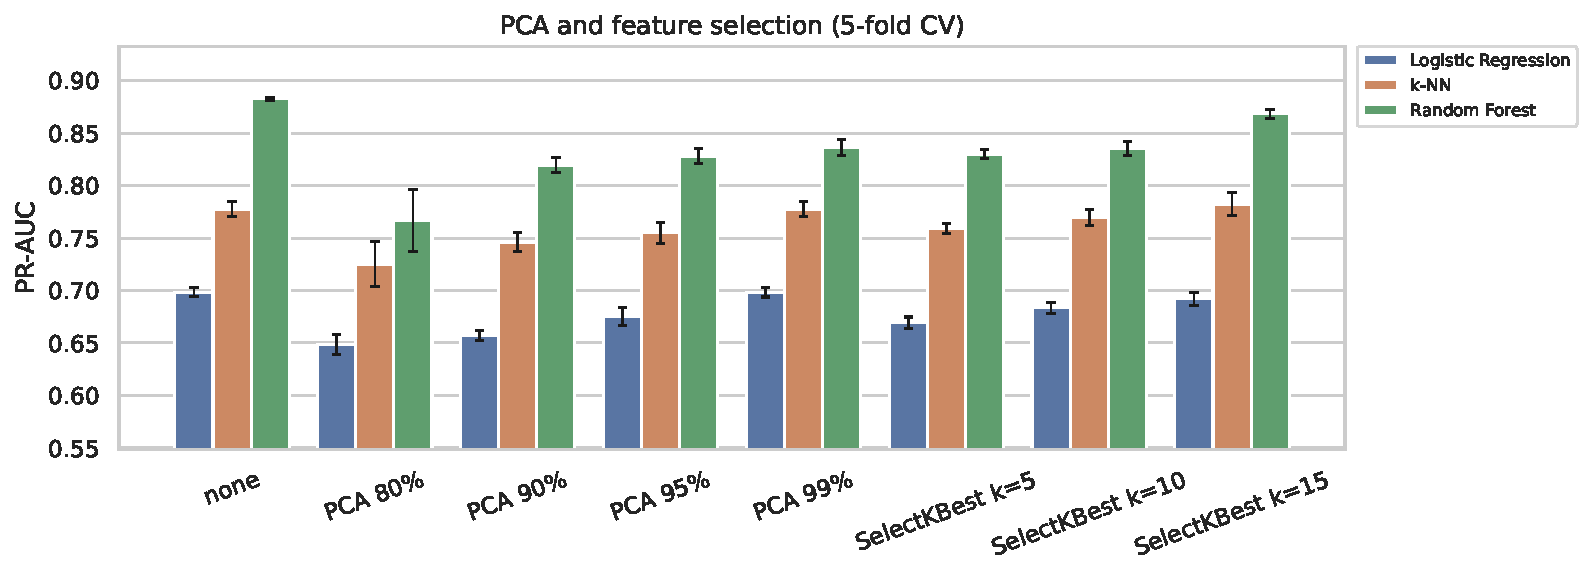
\includegraphics[width=0.9\linewidth]{suite_dimensionality.pdf}\caption{Dimensionality.}\label{fig:suite_dimensionality}\end{figure}
\subsubsection{Imbalance}
\begin{table}[H]
\centering
\scriptsize
\begin{adjustbox}{max width=\linewidth}
\begin{tabular}{llrrrrrr}
\toprule
model & imbalance & pr\_auc & sd & roc\_auc & f2 & recall & precision \\
\midrule
Logistic Regression & none & 0.7026 & 0.0039 & 0.8637 & 0.5390 & 0.5050 & 0.7381 \\
Logistic Regression & class\_weight & 0.6985 & 0.0045 & 0.8642 & 0.7063 & 0.7801 & 0.5125 \\
Logistic Regression & smote & 0.6983 & 0.0050 & 0.8638 & 0.7041 & 0.7750 & 0.5155 \\
Logistic Regression & undersample & 0.6983 & 0.0038 & 0.8641 & 0.7080 & 0.7822 & 0.5133 \\
Random Forest & none & 0.8843 & 0.0017 & 0.9314 & 0.7554 & 0.7152 & 0.9743 \\
Random Forest & class\_weight & 0.8827 & 0.0016 & 0.9313 & 0.7685 & 0.7392 & 0.9136 \\
Random Forest & smote & 0.8792 & 0.0023 & 0.9280 & 0.7568 & 0.7182 & 0.9641 \\
Random Forest & undersample & 0.8766 & 0.0016 & 0.9291 & 0.7809 & 0.7939 & 0.7334 \\
Hist. Gradient Boosting & none & 0.8982 & 0.0016 & 0.9440 & 0.7657 & 0.7265 & 0.9761 \\
Hist. Gradient Boosting & class\_weight & 0.8986 & 0.0029 & 0.9442 & 0.7923 & 0.7819 & 0.8370 \\
Hist. Gradient Boosting & smote & 0.8974 & 0.0016 & 0.9428 & 0.7678 & 0.7288 & 0.9766 \\
Hist. Gradient Boosting & undersample & 0.8928 & 0.0023 & 0.9406 & 0.7921 & 0.7962 & 0.7762 \\
\bottomrule
\end{tabular}
\end{adjustbox}
\caption{Class-imbalance strategies: 5-fold CV on the training set (F2, recall and precision at threshold 0.5).}
\label{tab:suite_imbalance}
\end{table}

\begin{figure}[H]\centering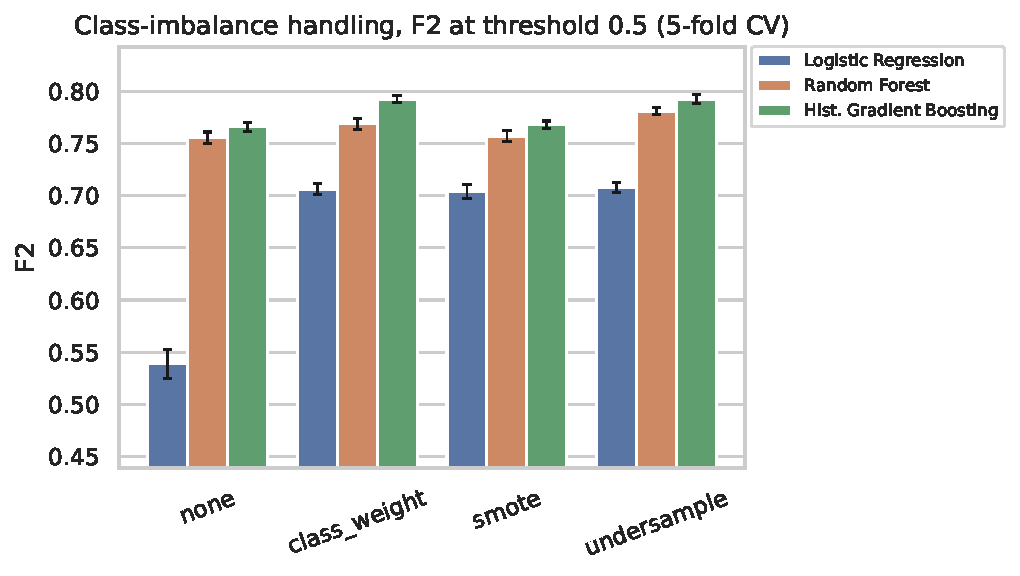
\includegraphics[width=0.9\linewidth]{suite_imbalance.pdf}\caption{Imbalance.}\label{fig:suite_imbalance}\end{figure}

\subsection{Tuned models}
\begin{table}[H]
\centering
\scriptsize
\begin{adjustbox}{max width=\linewidth}
\begin{tabular}{lp{5.4cm}rrrrr}
\toprule
model & best\_params & CV PR-AUC & sd & CV ROC-AUC & CV F2 & time (s) \\
\midrule
Logistic Regression & C=10, class\_weight=None & 0.7538 & 0.0072 & 0.8827 & 0.6247 & 3.6 \\
Linear SVM & C=1, class\_weight=None & 0.7473 & 0.0071 & 0.8801 & 0.6152 & 2.4 \\
SVM (RBF) & C=10, gamma=scale & 0.8501 & 0.0045 & 0.9115 & 0.7634 & 164.5 \\
k-NN & n\_neighbors=15, weights=distance & 0.8134 & 0.0058 & 0.8934 & 0.6459 & 12.5 \\
Gaussian Naive Bayes & var\_smoothing=0.001 & 0.6229 & 0.0120 & 0.8552 & 0.6077 & 0.9 \\
Decision Tree & class\_weight=None, max\_depth=10, min\_samples\_leaf=20 & 0.8598 & 0.0040 & 0.9151 & 0.7438 & 5.6 \\
Random Forest & class\_weight=None, max\_features=0.5, min\_samples\_leaf=3 & 0.8902 & 0.0025 & 0.9341 & 0.7526 & 198.4 \\
Hist. Gradient Boosting & class\_weight=None, learning\_rate=0.05, max\_iter=300, max\_leaf\_nodes=31 & 0.8988 & 0.0026 & 0.9441 & 0.7656 & 22.1 \\
\bottomrule
\end{tabular}
\end{adjustbox}
\caption{Grid-search results (5-fold CV, refit on PR-AUC; F2 at threshold 0.5).}
\label{tab:tuning}
\end{table}

\begin{table}[H]
\centering
\small
\begin{adjustbox}{max width=\linewidth}
\begin{tabular}{lrrrrrrr}
\toprule
model & pr\_auc & roc\_auc & threshold & F2 & recall & precision & accuracy \\
\midrule
Hist. Gradient Boosting & \textbf{0.9045} & \textbf{0.9459} & 0.1515 & \textbf{0.8132} & \textbf{0.8512} & 0.6901 & 0.8839 \\
Random Forest & 0.8934 & 0.9361 & 0.2222 & 0.8021 & 0.8068 & 0.7841 & 0.9092 \\
Decision Tree & 0.8623 & 0.9180 & 0.1414 & 0.7670 & 0.7856 & 0.7006 & 0.8797 \\
SVM (RBF) & 0.8561 & 0.9147 & -0.4900 & 0.7703 & 0.8117 & 0.6398 & 0.8589 \\
k-NN & 0.8163 & 0.8925 & 0.2424 & 0.7501 & 0.7906 & 0.6228 & 0.8495 \\
Logistic Regression & 0.7512 & 0.8797 & 0.2224 & 0.7360 & 0.7955 & 0.5665 & 0.8222 \\
Linear SVM & 0.7443 & 0.8774 & -0.4521 & 0.7339 & 0.7962 & 0.5589 & 0.8180 \\
Gaussian Naive Bayes & 0.6244 & 0.8503 & 0.0101 & 0.7140 & 0.8096 & 0.4850 & 0.7704 \\
\bottomrule
\end{tabular}
\end{adjustbox}
\caption{Test-set results of the tuned traditional models; F2, recall, precision and accuracy at the F2-tuned threshold.}
\label{tab:test_traditional}
\end{table}

\begin{figure}[H]\centering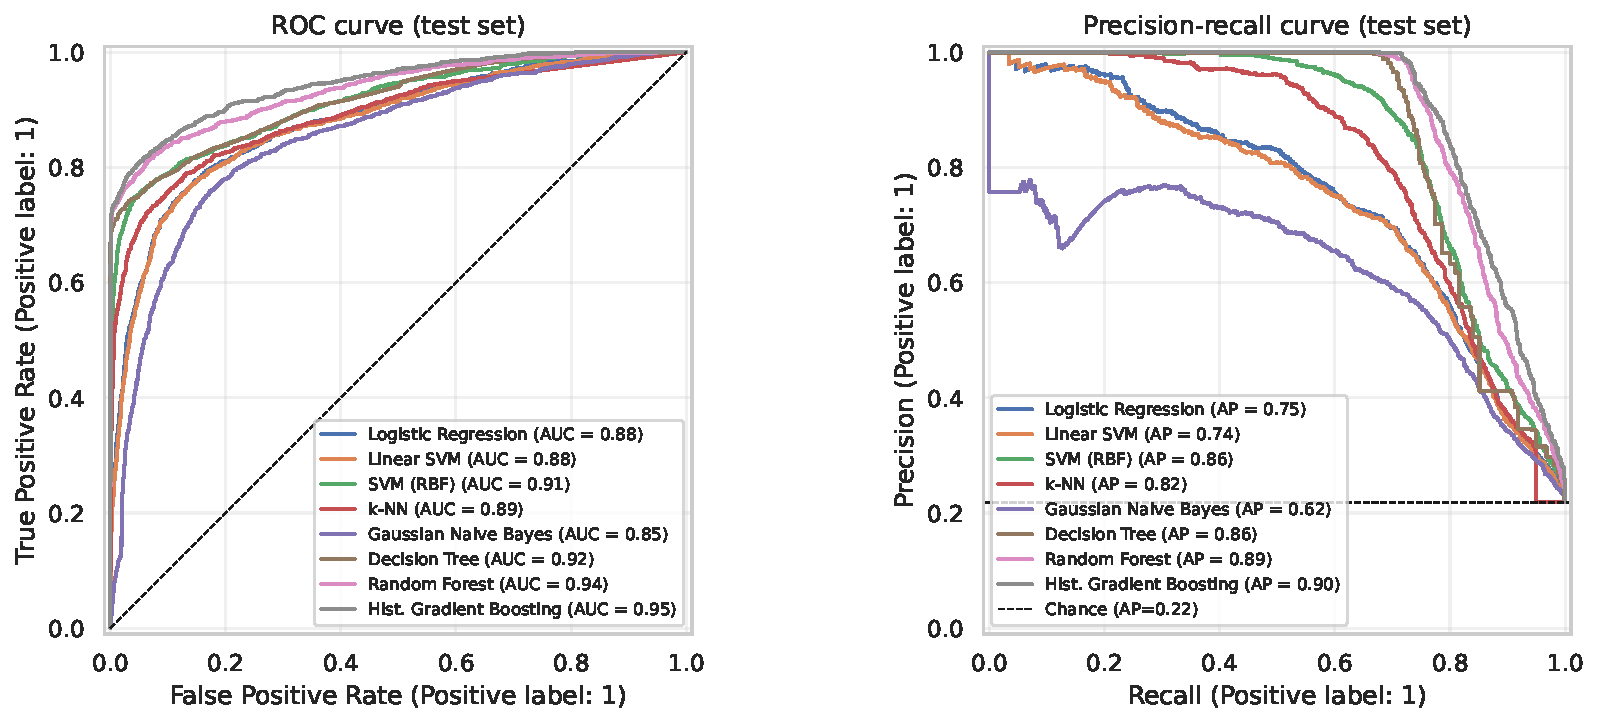
\includegraphics[width=\linewidth]{roc_pr_traditional.pdf}\caption{ROC.}\label{fig:roc_trad}\end{figure}
\begin{figure}[H]\centering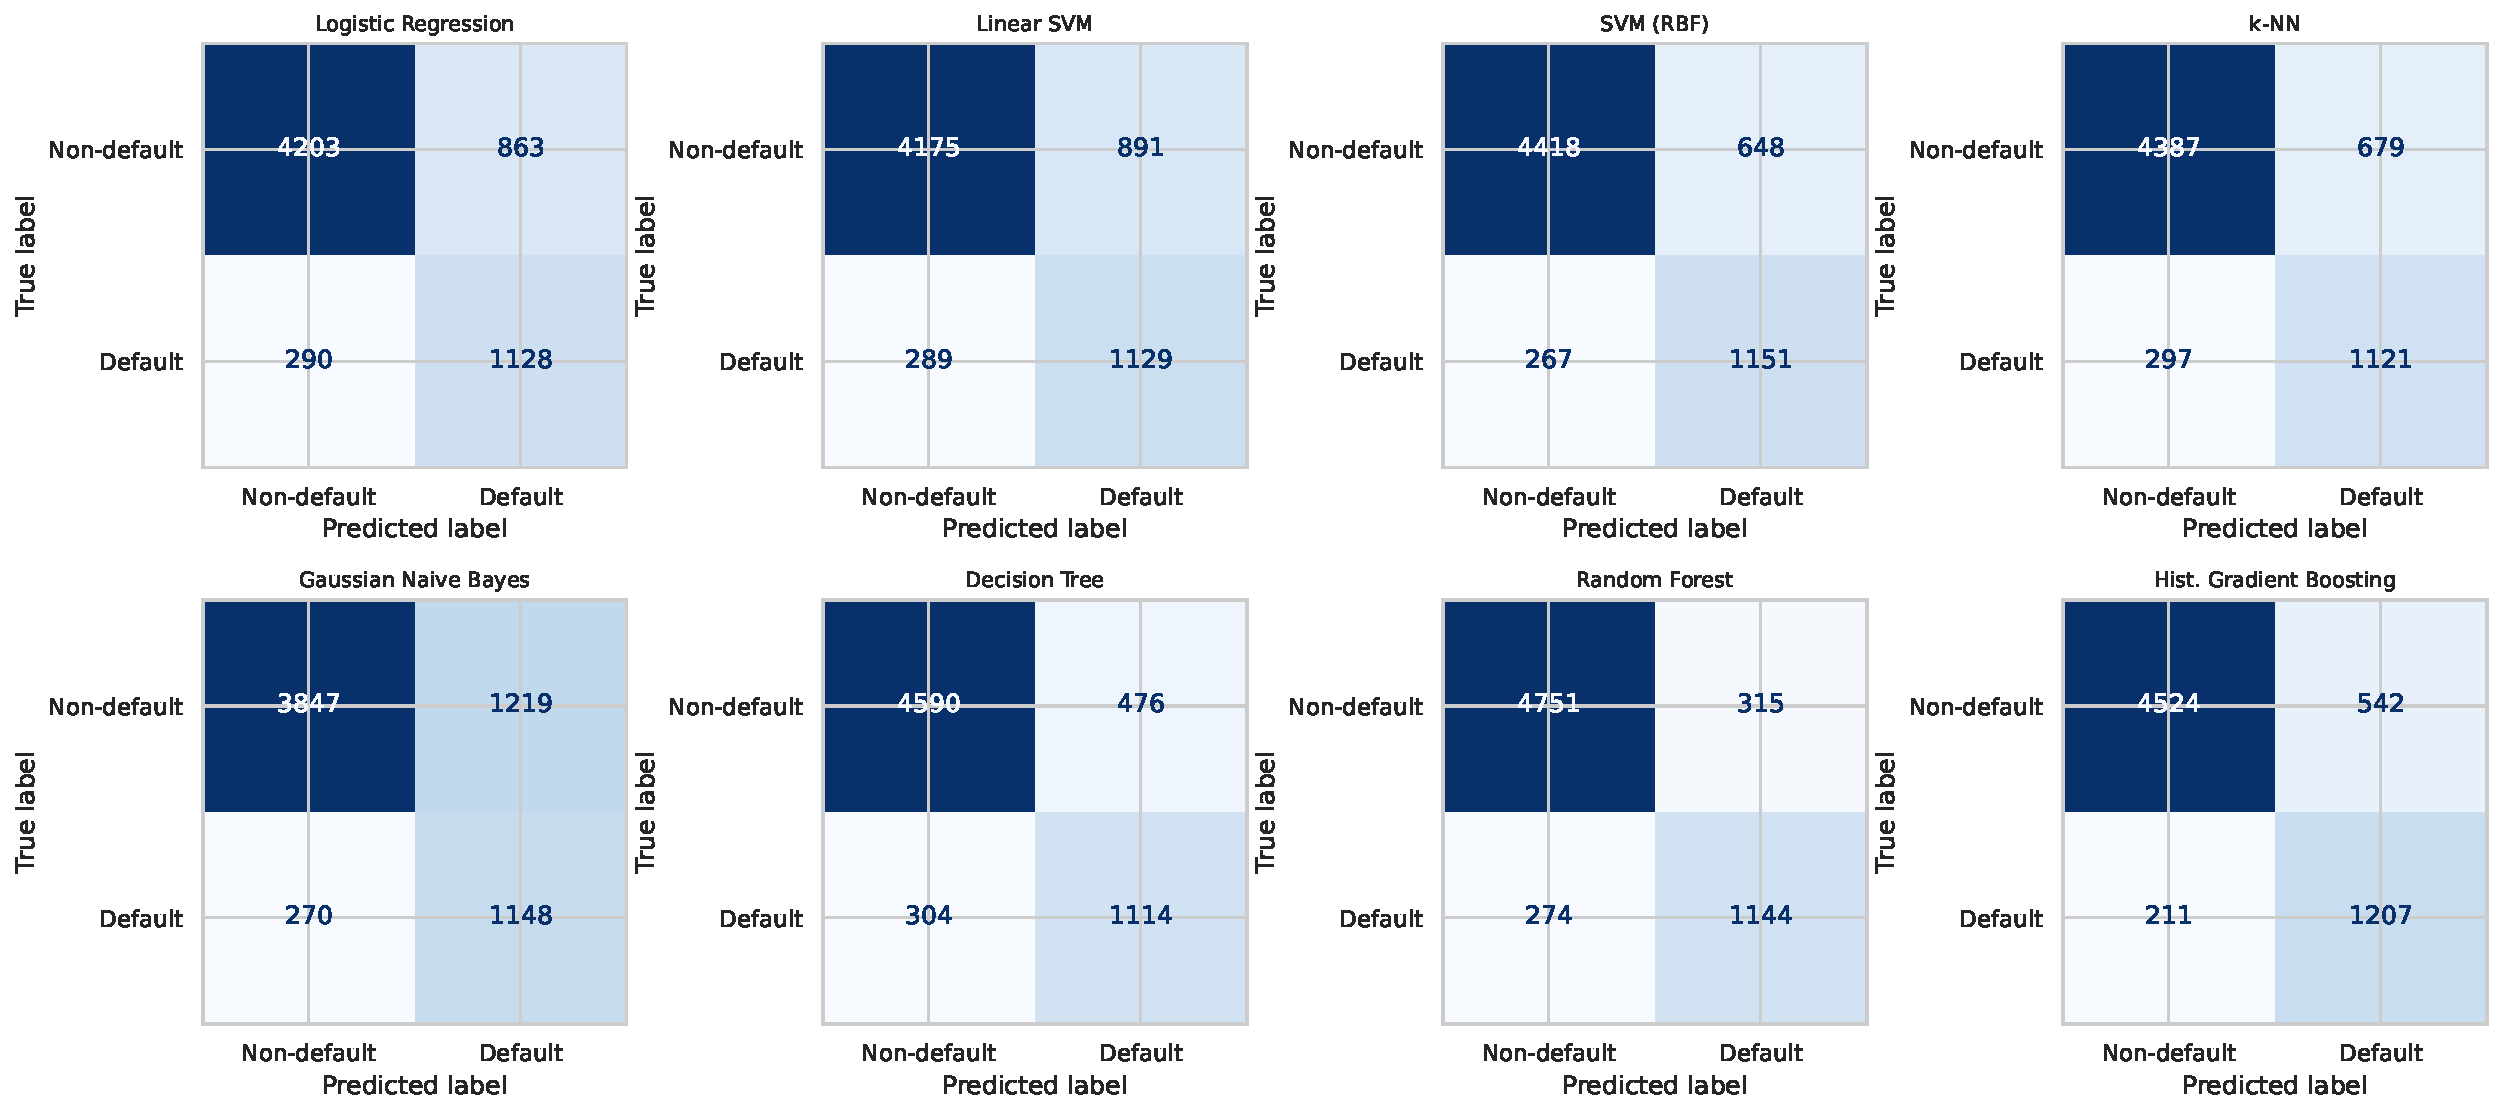
\includegraphics[width=\linewidth]{confusion_traditional.pdf}\caption{Confusion.}\label{fig:confusion}\end{figure}
\begin{figure}[H]\centering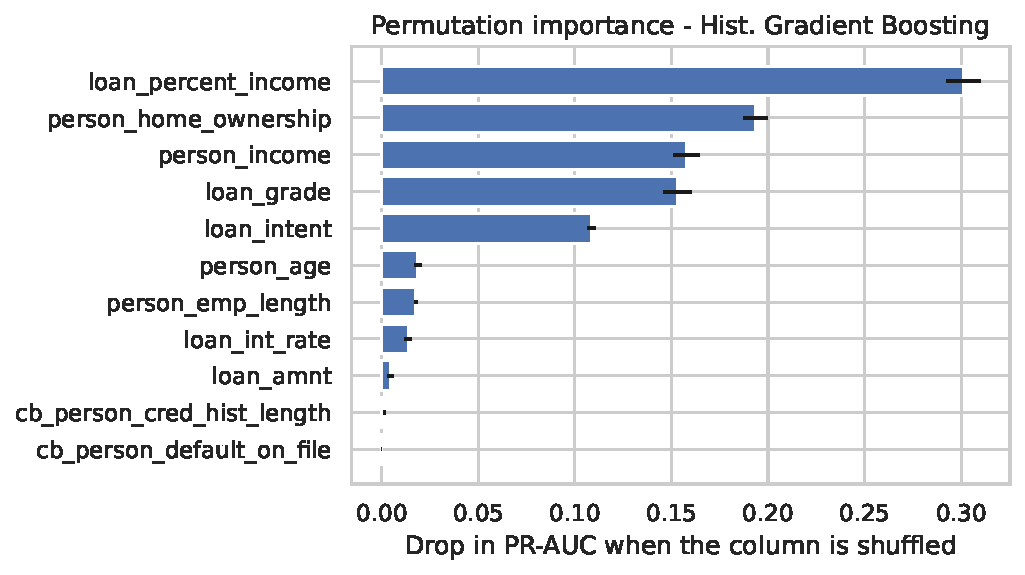
\includegraphics[width=0.7\linewidth]{importance_best.pdf}\caption{Importance.}\label{fig:importance}\end{figure}

\subsection{Deep learning}
\begin{table}[H]
\centering
\scriptsize
\begin{adjustbox}{max width=\linewidth}
\begin{tabular}{lrrrrrrr}
\toprule
model & val PR-AUC & pr\_auc & roc\_auc & F2 & recall & epochs & time (s) \\
\midrule
MLP 128-64 (reference) & 0.8729 & 0.8640 & 0.9221 & 0.7616 & 0.7955 & 69 & 9.9 \\
MLP 64-32 (smaller) & 0.8693 & 0.8633 & 0.9223 & 0.7623 & 0.7743 & 63 & 6.0 \\
MLP 256-128-64 (deeper) & 0.8724 & 0.8658 & 0.9226 & 0.7651 & 0.7913 & 40 & 9.7 \\
No dropout & 0.8662 & 0.8619 & 0.9213 & 0.7659 & 0.7948 & 49 & 3.8 \\
One-hot instead of embeddings & 0.8709 & 0.8647 & 0.9214 & 0.7634 & 0.7736 & 81 & 8.4 \\
No class weighting & 0.8712 & 0.8633 & 0.9201 & 0.7572 & 0.7898 & 47 & 5.1 \\
No engineered features & 0.8671 & 0.8605 & 0.9196 & 0.7627 & 0.8004 & 39 & 4.2 \\
\bottomrule
\end{tabular}
\end{adjustbox}
\caption{MLP variants: validation PR-AUC (used for selection) and test metrics.}
\label{tab:mlp}
\end{table}

\begin{table}[H]
\centering
\small
\begin{adjustbox}{max width=\linewidth}
\begin{tabular}{lrrrrrrr}
\toprule
model & pr\_auc & roc\_auc & F2 & recall & precision & accuracy & time (s) \\
\midrule
MLP 128-64 (reference) & 0.8619 $\pm$ 0.0017 & 0.9200 $\pm$ 0.0017 & 0.7621 $\pm$ 0.0017 & 0.7956 $\pm$ 0.0088 & 0.6535 $\pm$ 0.0283 & 0.8626 $\pm$ 0.0105 & 6.8 \\
TabNet & 0.8612 $\pm$ 0.0026 & 0.9180 $\pm$ 0.0014 & 0.7568 $\pm$ 0.0039 & 0.7984 $\pm$ 0.0170 & 0.6288 $\pm$ 0.0398 & 0.8517 $\pm$ 0.0148 & 34.0 \\
\bottomrule
\end{tabular}
\end{adjustbox}
\caption{Deep learning models on the test set, mean $\pm$ sd over 5 seeds (threshold tuned for F2 on a validation split; training time per seed).}
\label{tab:deep}
\end{table}

\begin{figure}[H]\centering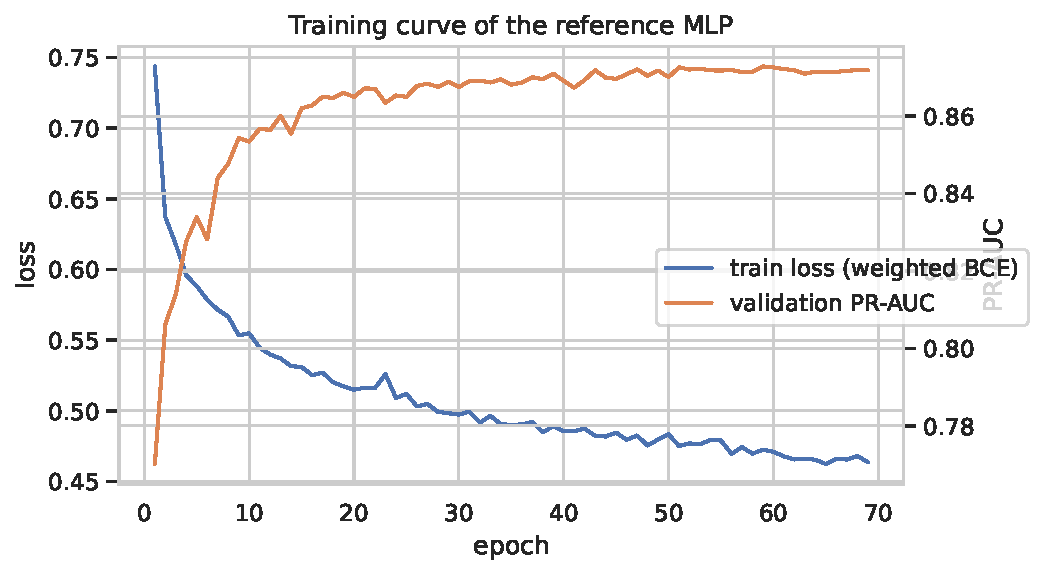
\includegraphics[width=0.6\linewidth]{mlp_training.pdf}\caption{MLP.}\label{fig:mlp_training}\end{figure}
\begin{figure}[H]\centering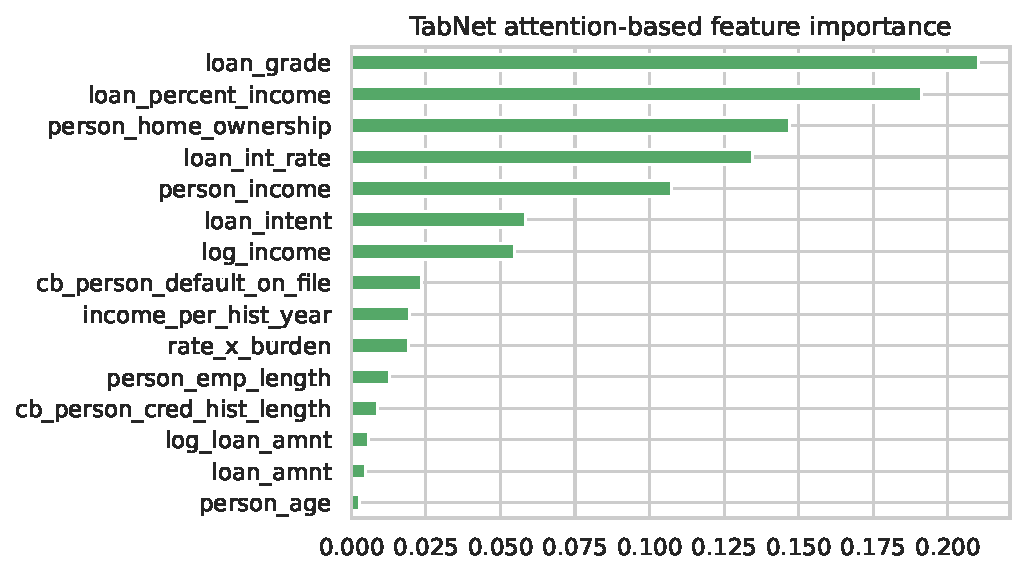
\includegraphics[width=0.6\linewidth]{tabnet_importance.pdf}\caption{TabNet.}\label{fig:tabnet}\end{figure}
\begin{figure}[H]\centering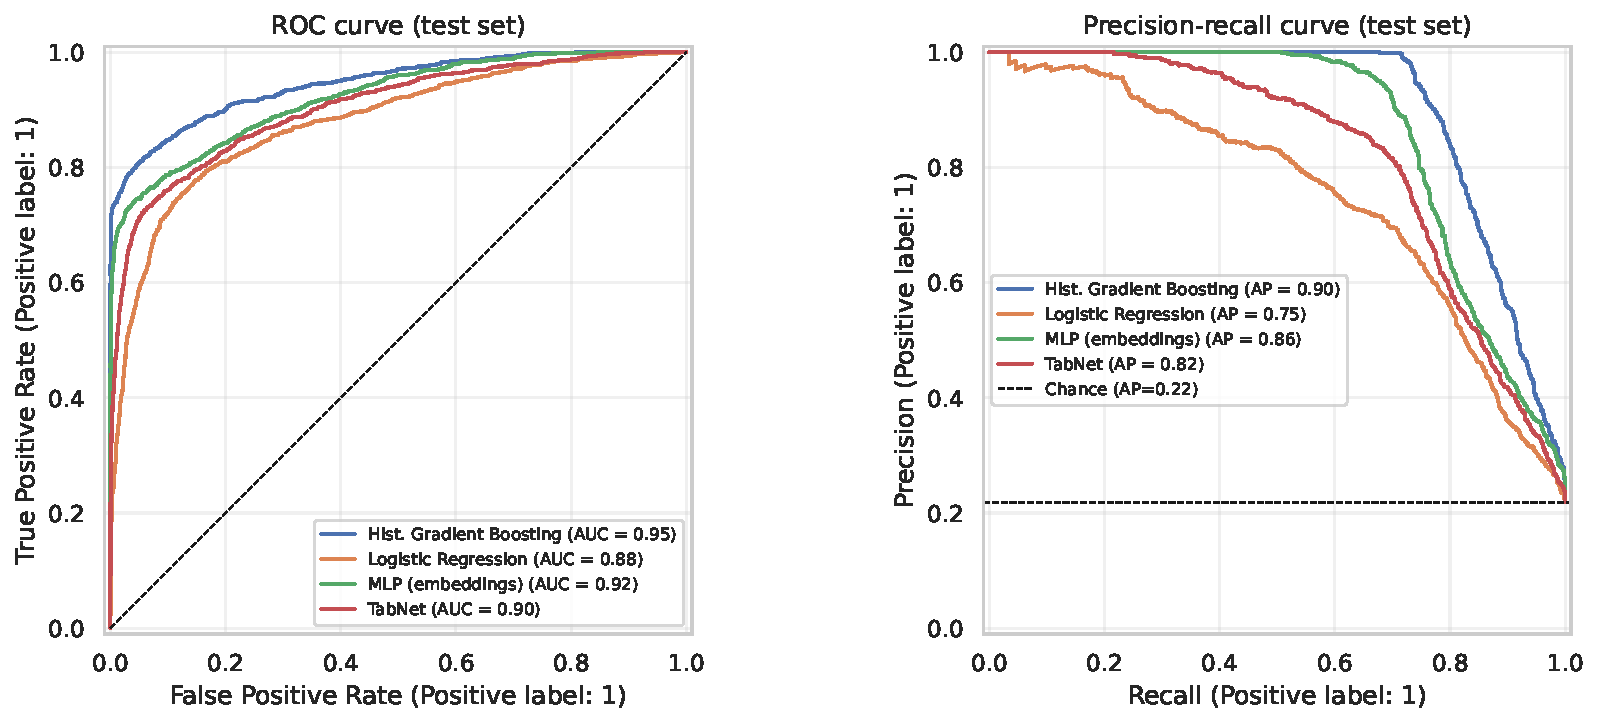
\includegraphics[width=\linewidth]{roc_pr_traditional_vs_deep.pdf}\caption{Trad vs deep.}\label{fig:roc_deep}\end{figure}

\subsection{Bayesian network}
\begin{table}[H]
\centering
\small
\begin{adjustbox}{max width=\linewidth}
\begin{tabular}{rrrrrr}
\toprule
n\_bins & alpha & Expert DAG & Hill-climb BIC & Naive Bayes & TAN \\
\midrule
3 & 0.1 & 0.7024 & 0.6088 & 0.6251 & 0.7401 \\
3 & 1 & 0.7015 & 0.6111 & 0.6249 & 0.7393 \\
3 & 10 & 0.6912 & 0.6114 & 0.6261 & 0.7312 \\
5 & 0.1 & 0.7338 & 0.6479 & 0.6633 & 0.7672 \\
5 & 1 & 0.7316 & 0.6479 & 0.6649 & 0.7656 \\
5 & 10 & 0.7111 & 0.6457 & 0.6645 & 0.7578 \\
8 & 0.1 & 0.7948 & 0.6859 & 0.6905 & 0.7915 \\
8 & 1 & 0.7908 & 0.6879 & 0.6919 & 0.7893 \\
8 & 10 & 0.7674 & 0.6871 & 0.6916 & 0.7787 \\
12 & 0.1 & 0.7940 & 0.7416 & 0.6940 & 0.7542 \\
12 & 1 & 0.7915 & 0.7416 & 0.6956 & 0.7515 \\
12 & 10 & 0.7780 & 0.7383 & 0.6954 & 0.7403 \\
\bottomrule
\end{tabular}
\end{adjustbox}
\caption{Bayesian networks: validation PR-AUC by number of bins and Dirichlet pseudo-count $\alpha$.}
\label{tab:bn_sens}
\end{table}

\begin{table}[H]
\centering
\scriptsize
\begin{adjustbox}{max width=\linewidth}
\begin{tabular}{lrrrrrrrrrrr}
\toprule
structure & bins & alpha & edges & parameters & test log-lik. & pr\_auc & roc\_auc & F2 & recall & precision & accuracy \\
\midrule
Expert DAG & 8 & 0.1 & 12 & 2041 & -100750 & 0.7822 & 0.8712 & 0.7152 & 0.7736 & 0.5493 & 0.8117 \\
Hill-climb BIC & 12 & 0.1 & 17 & 3736 & -103692 & 0.7332 & 0.8579 & 0.7033 & 0.7941 & 0.4826 & 0.7688 \\
Naive Bayes & 12 & 1 & 11 & 171 & -136946 & 0.7061 & 0.8635 & 0.7149 & 0.7962 & 0.5076 & 0.7866 \\
TAN & 8 & 0.1 & 21 & 777 & -105532 & \textbf{0.7895} & \textbf{0.8900} & 0.7390 & 0.8110 & 0.5453 & 0.8108 \\
\bottomrule
\end{tabular}
\end{adjustbox}
\caption{Bayesian-network structures on the test set, each with the bins and $\alpha$ selected on validation data.}
\label{tab:bn_results}
\end{table}

\begin{figure}[H]\centering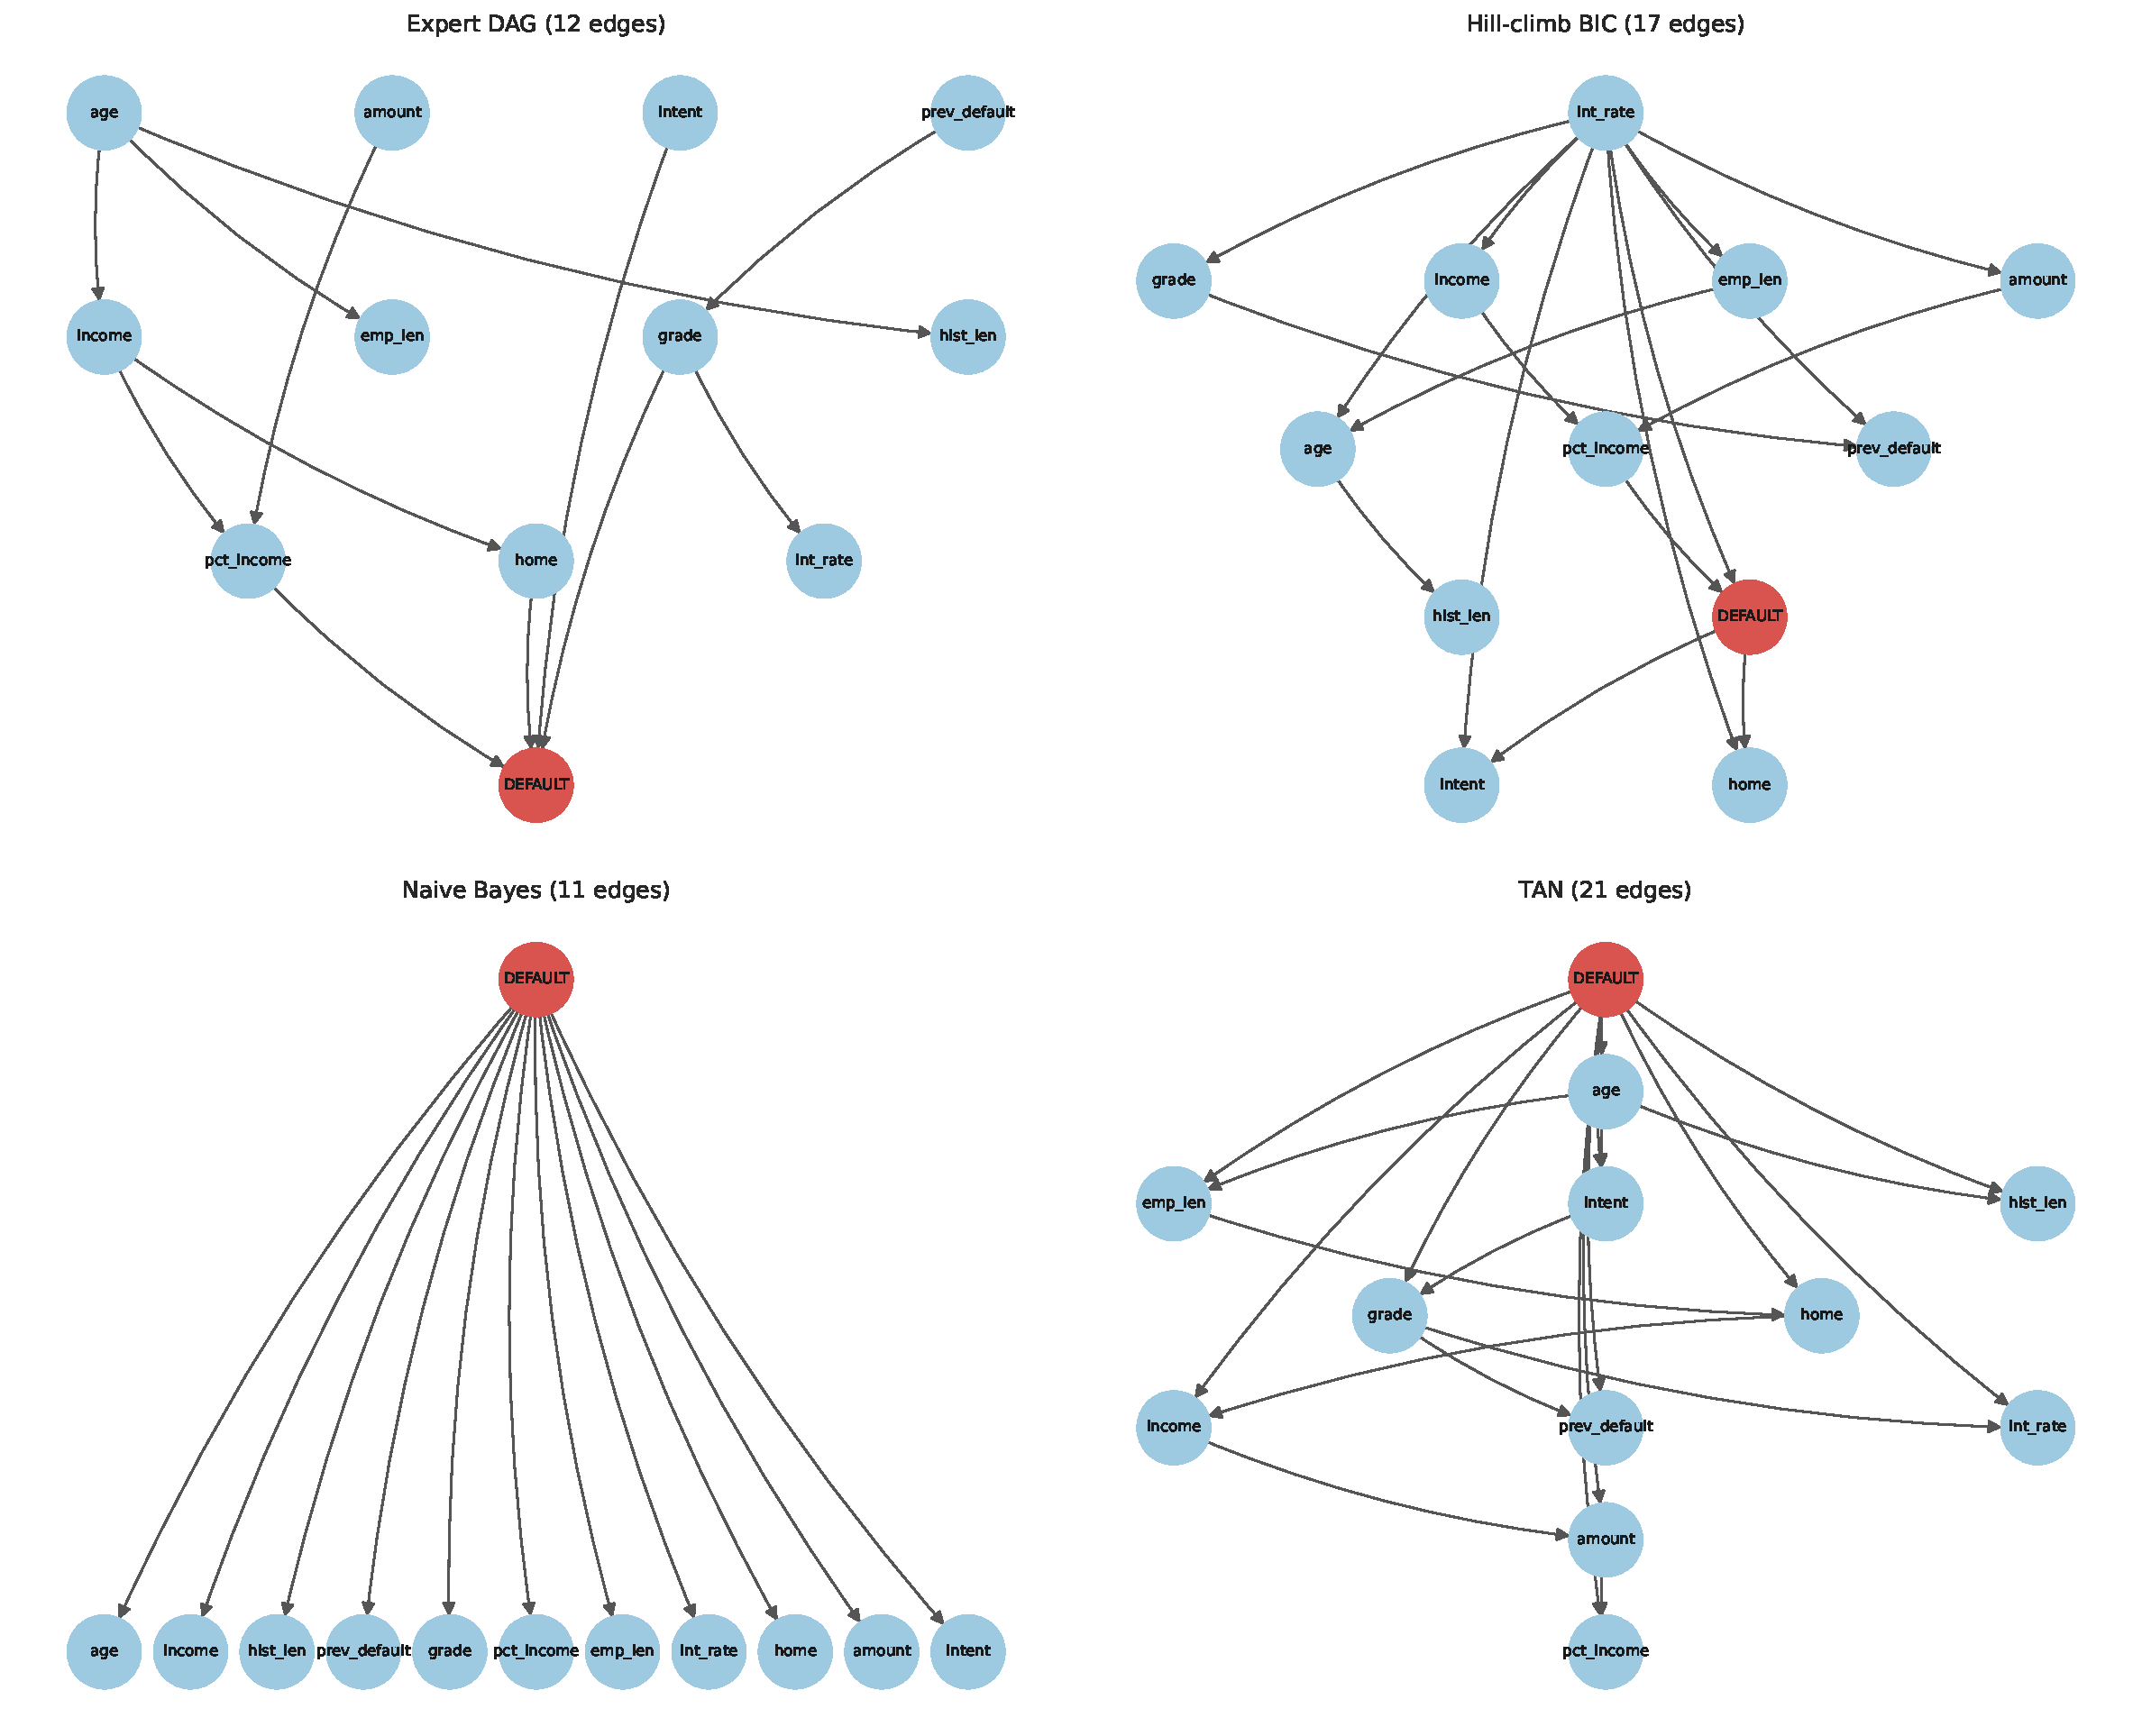
\includegraphics[width=\linewidth]{bn_structures.pdf}\caption{Structures.}\label{fig:bn_structures}\end{figure}
\begin{figure}[H]\centering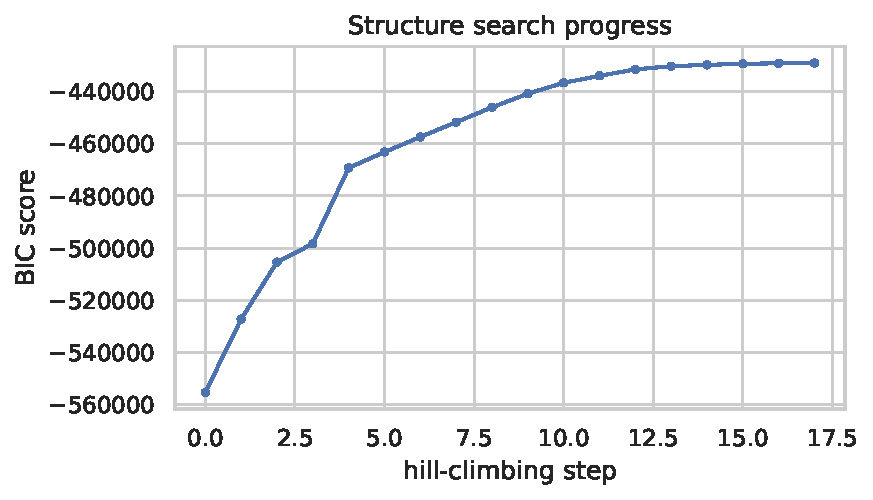
\includegraphics[width=0.6\linewidth]{bn_bic_trace.pdf}\caption{BIC.}\label{fig:bic}\end{figure}
\begin{table}[H]
\centering
\small
\begin{adjustbox}{max width=\linewidth}
\begin{tabular}{lrrrr}
\toprule
query & empirical & support & TAN & Expert DAG \\
\midrule
P(default) & 0.2187 & 25932 & 0.2187 & 0.2594 \\
P(default \textbar{} grade=A) & 0.0998 & 8584 & 0.0998 & 0.1750 \\
P(default \textbar{} grade=D) & 0.5902 & 2889 & 0.5900 & 0.5749 \\
P(default \textbar{} grade=G) & 0.9792 & 48 & 0.9675 & 0.6361 \\
P(default \textbar{} home=RENT) & 0.3167 & 13114 & 0.3149 & 0.3675 \\
P(default \textbar{} home=OWN) & 0.0715 & 2042 & 0.0681 & 0.1696 \\
P(default \textbar{} grade=D, home=OWN) & 0.0463 & 216 & 0.2731 & 0.0780 \\
P(default \textbar{} intent=MEDICAL) & 0.2672 & 4842 & 0.2672 & 0.3008 \\
P(default \textbar{} intent=VENTURE) & 0.1505 & 4610 & 0.1506 & 0.1901 \\
P(prev\_default=Y \textbar{} default=1) & 0.3063 & 5671 & 0.3064 & 0.2685 \\
P(prev\_default=Y \textbar{} default=0) & 0.1404 & 20261 & 0.1404 & 0.1445 \\
P(grade in D..G \textbar{} default=1) & 0.4195 & 5671 & 0.4196 & 0.3408 \\
P(grade in D..G \textbar{} default=0) & 0.0746 & 20261 & 0.0747 & 0.0832 \\
\bottomrule
\end{tabular}
\end{adjustbox}
\caption{Exact answers of two networks (variable elimination) against the empirical frequency in the training data; support is the number of training rows matching the evidence.}
\label{tab:bn_queries}
\end{table}

\begin{table}[H]
\centering
\small
\begin{adjustbox}{max width=\linewidth}
\begin{tabular}{lrrrr}
\toprule
method & samples & MAE, 2 evid. & MAE, 5 evid. & MAE, 10 evid. \\
\midrule
Gibbs sampling & 100 & 0.0444 & 0.0353 & 0.0159 \\
Gibbs sampling & 1000 & 0.0154 & 0.0124 & 0.0057 \\
Gibbs sampling & 10000 & 0.0061 & 0.0043 & 0.0025 \\
Likelihood weighting & 100 & 0.0467 & 0.0356 & 0.0183 \\
Likelihood weighting & 1000 & 0.0160 & 0.0131 & 0.0057 \\
Likelihood weighting & 10000 & 0.0049 & 0.0030 & 0.0015 \\
Rejection sampling & 100 & 0.1636 & 0.3041 & 0.3868 \\
Rejection sampling & 1000 & 0.0639 & 0.2514 & 0.3868 \\
Rejection sampling & 10000 & 0.0178 & 0.1673 & 0.3788 \\
\bottomrule
\end{tabular}
\end{adjustbox}
\caption{Mean absolute error of approximate $P(\text{default} \mid \bm{e})$ against variable elimination (60 random test applicants per evidence size).}
\label{tab:bn_inference}
\end{table}

\begin{table}[H]
\centering
\small
\begin{adjustbox}{max width=\linewidth}
\begin{tabular}{rrrr}
\toprule
samples & 2 evidence vars & 5 evidence vars & 10 evidence vars \\
\midrule
100 & 0.04900 & 0.00100 & 0.00000 \\
1000 & 0.04502 & 0.00077 & 0.00000 \\
10000 & 0.04685 & 0.00073 & 0.00000 \\
\bottomrule
\end{tabular}
\end{adjustbox}
\caption{Acceptance rate of rejection sampling.}
\label{tab:bn_acceptance}
\end{table}

\begin{figure}[H]\centering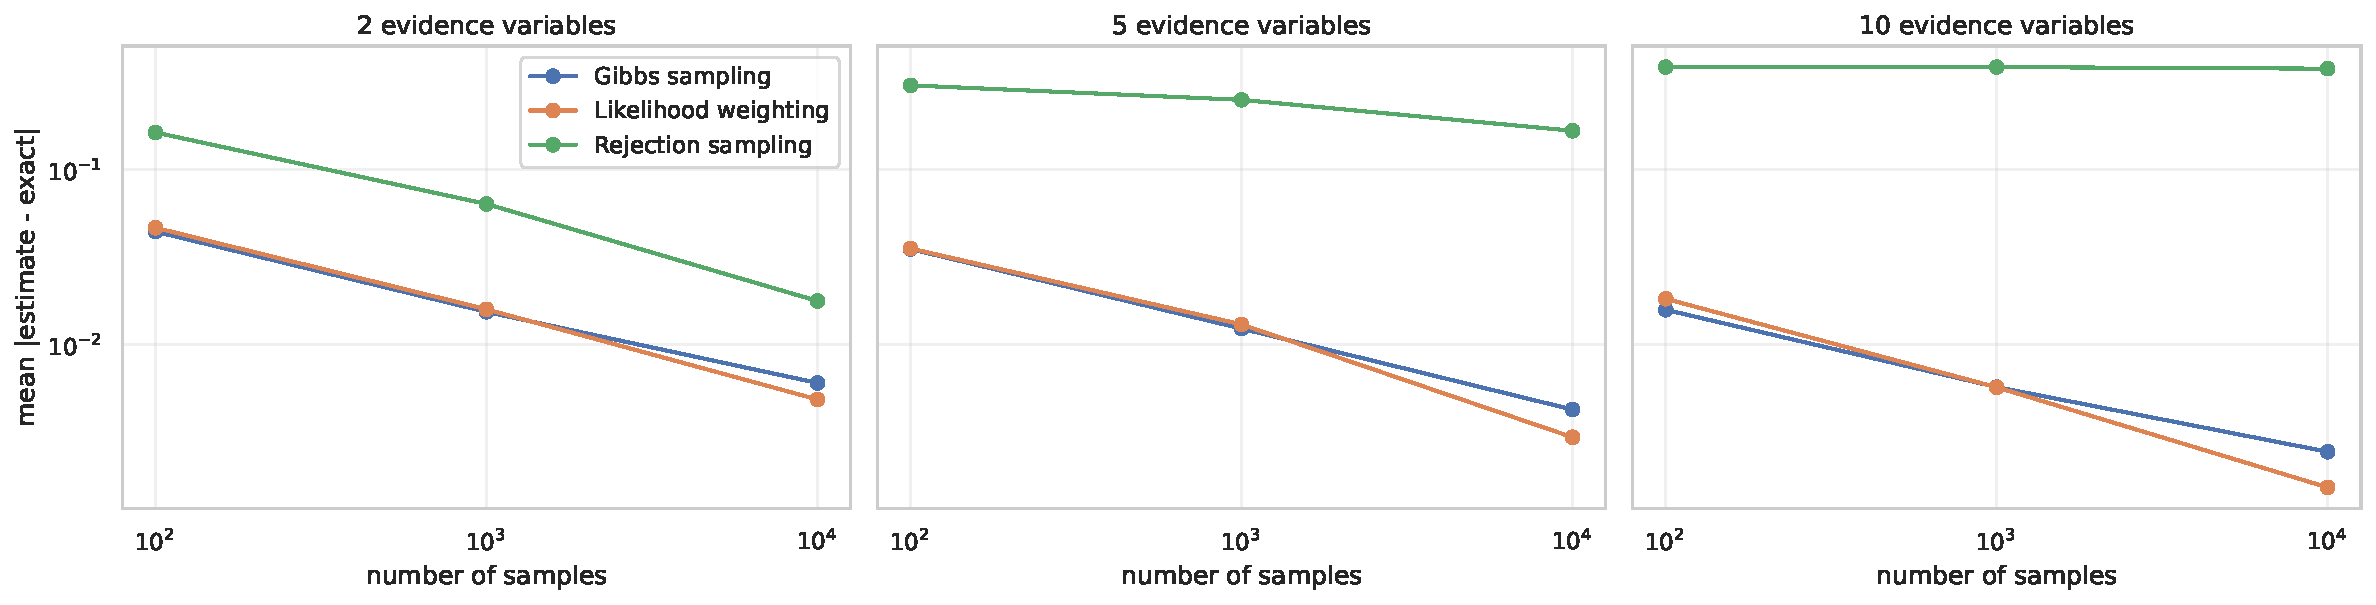
\includegraphics[width=\linewidth]{bn_inference_error.pdf}\caption{Inference.}\label{fig:bn_inference}\end{figure}

\subsection{Overall}
\begin{table}[H]
\centering
\small
\begin{adjustbox}{max width=\linewidth}
\begin{tabular}{llrrrrrr}
\toprule
family & model & pr\_auc & roc\_auc & f2 & recall & precision & accuracy \\
\midrule
Traditional & Hist. Gradient Boosting & \textbf{0.9045} & \textbf{0.9459} & \textbf{0.8132} & \textbf{0.8512} & 0.6901 & 0.8839 \\
Traditional & Random Forest & 0.8934 & 0.9361 & 0.8021 & 0.8068 & 0.7841 & 0.9092 \\
Traditional & Decision Tree & 0.8623 & 0.9180 & 0.7670 & 0.7856 & 0.7006 & 0.8797 \\
Deep learning & MLP (entity embeddings) & 0.8619 $\pm$ 0.0017 & 0.9200 $\pm$ 0.0017 & 0.7621 $\pm$ 0.0017 & 0.7956 $\pm$ 0.0088 & 0.6535 $\pm$ 0.0283 & 0.8626 $\pm$ 0.0105 \\
Deep learning & TabNet & 0.8612 $\pm$ 0.0026 & 0.9180 $\pm$ 0.0014 & 0.7568 $\pm$ 0.0039 & 0.7984 $\pm$ 0.0170 & 0.6288 $\pm$ 0.0398 & 0.8517 $\pm$ 0.0148 \\
Traditional & SVM (RBF) & 0.8561 & 0.9147 & 0.7703 & 0.8117 & 0.6398 & 0.8589 \\
Traditional & k-NN & 0.8163 & 0.8925 & 0.7501 & 0.7906 & 0.6228 & 0.8495 \\
Bayesian network & BN - TAN & 0.7895 & 0.8900 & 0.7390 & 0.8110 & 0.5453 & 0.8108 \\
Bayesian network & BN - Expert DAG & 0.7822 & 0.8712 & 0.7152 & 0.7736 & 0.5493 & 0.8117 \\
Traditional & Logistic Regression & 0.7512 & 0.8797 & 0.7360 & 0.7955 & 0.5665 & 0.8222 \\
Traditional & Linear SVM & 0.7443 & 0.8774 & 0.7339 & 0.7962 & 0.5589 & 0.8180 \\
Bayesian network & BN - Hill-climb BIC & 0.7332 & 0.8579 & 0.7033 & 0.7941 & 0.4826 & 0.7688 \\
Bayesian network & BN - Naive Bayes & 0.7061 & 0.8635 & 0.7149 & 0.7962 & 0.5076 & 0.7866 \\
Traditional & Gaussian Naive Bayes & 0.6244 & 0.8503 & 0.7140 & 0.8096 & 0.4850 & 0.7704 \\
\bottomrule
\end{tabular}
\end{adjustbox}
\caption{All model families on the test set, ranked by PR-AUC (F2, recall, precision and accuracy at the tuned threshold); deep models are mean $\pm$ sd over 5 seeds.}
\label{tab:overall}
\end{table}

\begin{figure}[H]\centering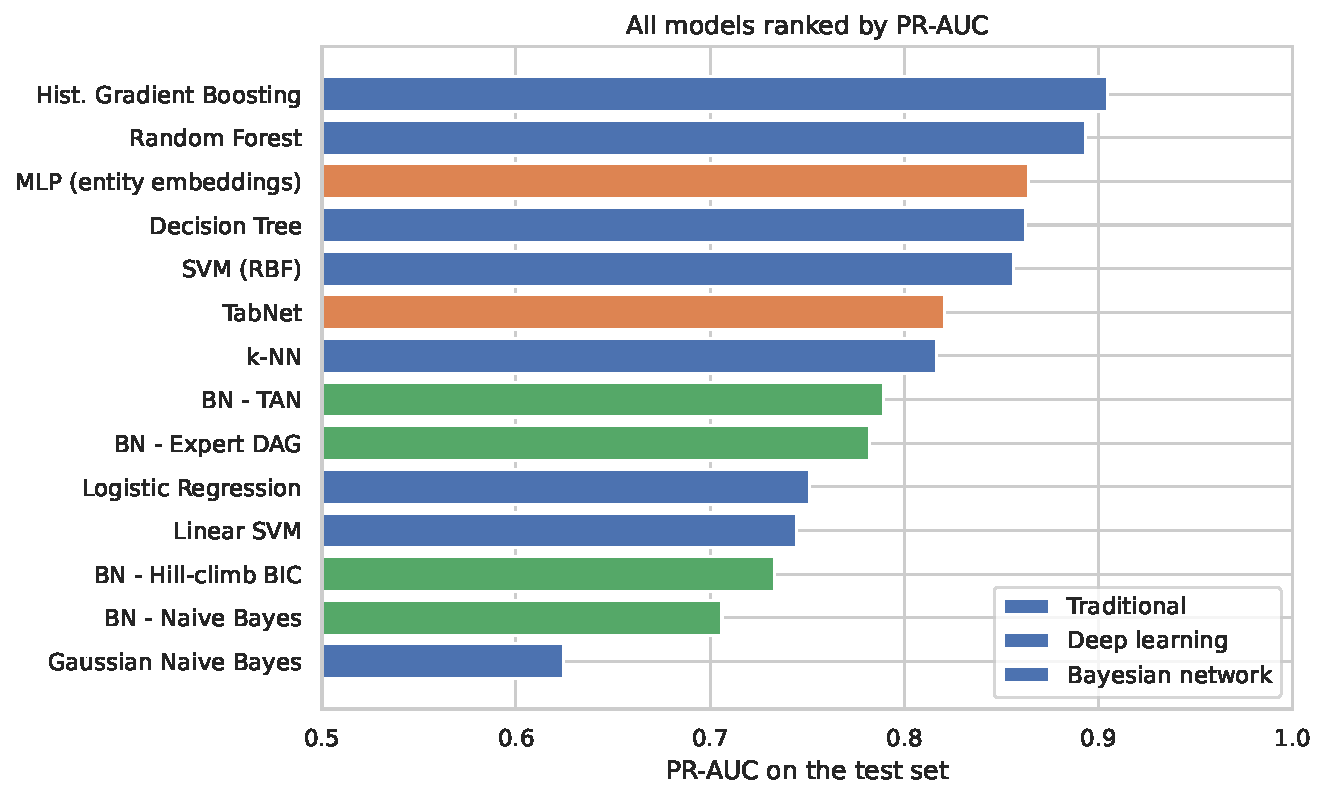
\includegraphics[width=0.8\linewidth]{overall_pr_auc.pdf}\caption{Overall.}\label{fig:overall}\end{figure}
Best: \BestModel{} \BestPrAuc{} \BestFTwo{} \BnBins{} \VeMs{}.
